\chapter{Employing GPUs in scientific algorithms}

The information age has brought a massive increase in the amount of data that is being collected and processed. The `data explosion' can be observed in virtually every field of computer science. In the scientific domain, this phenomenon is multiplied by increasingly powerful data-gathering devices (i.e., cytometers in bioinformatics, optic sensors in physics, seismometers in geology, etc.). The amount of data is simply too large to be processed in the required time. In order to alleviate this apparent pressure, the corresponding algorithm (which typically has super-linear time complexity) must be ported to massively parallel architectures, such as GPUs. The provided advantage can result in the ability to assess bigger data, use more detailed processing methods, or analyze the data in real time.

This chapter enumerates four selected scientific algorithms and discusses their challenges in porting to GPUs to enable higher performance.

\section{Hierarchical clustering with the Ma\-ha\-la\-no\-bis linkage}

In the field of bioinformatics, hierarchical clustering is a popular method for analyzing various types of data. 
In general, hierarchical clustering is an unsupervised machine learning method that aims to group the data points into clusters according to some \emph{linkage criterion}.
Clustering is an iterative method that begins with each data point interpreted as a single cluster and, in each iteration, the two most similar clusters are merged with respect to a linkage criterion until a single cluster remains.
There are many cluster linkage criteria used in the field, each with advantages and disadvantages. 
Perhaps the most common linkage may be the \emph{centroid linkage}, which defines cluster similarity as the distance between their centroids (the mean points). In the domain of bioinformatics, hierarchical clustering with the \emph{Mahalanobis linkage} is used, which is a more sophisticated method suitable for analyzing multidimensional single-cell cytometry datasets.

\subsection{Background}

Mahalanobis hierarchical clustering was proposed by Fišer et al.~\cite{fivser2012detection} as a valuable tool for analysis of flow cytometry datasets. Due to the ever increasing rate of data acquisition, the size of flow cytometry datasets is constantly growing. Modern flow cytometers are able to process samples with millions of cells and measure tens of parameters (point dimensions) simultaneously. More traditional methods, such as manual gating, are not suitable for such high-dimensional data and are heavily observer-dependent. Automated hierarchical clustering methods offer a viable solution but often fail to reflect the elliptical shapes of flow cytometric populations. 

For this purpose, the authors proposed the Mahalanobis linkage. This allows for a very natural formation of clusters in biological data. However, the benefits come at a cost of a high time and space complexity. The author claim the upper usable bound of dataset size to be $10^4$ using the original \texttt{C} application. They state that the quadratic space complexity makes for the most significant limiting factor, leaving it unfeasible to analyze bigger datasets on current desktop computers.

The authors tried to alleviate this limitation by implementing the approximation of \emph{apriori clusters}, where the data was pre-clustered using a naive euclidean-based linkage reducing the overall size of the dataset. This increased the usability of the original code to datasets of around $10^6$ data points within an interactive environment~\cite{kratochvil2020shinysom}. Still, the proposed optimization could not keep up with the contemporary data aquisition methods, generating datasets of millions of multidimensional data points.

\subsection{Algorithm complexity}

Mahalanobis linkage uses \emph{Mahalanobis distance}~\cite{mahalanobis1936generalized} to measure the similarity between clusters:
\begin{defn}[Mahalanobis distance]
    Suppose a probability distribution $C$ on $\R^d$ with mean $\bar{C} \in \R^d$ and a convariance matrix $\cov(C)$. If the matrix $\cov(C)$ is regular, we define the \emph{Mahalanobis distance} between $u \in \R^d$ and $C$ as
    \begin{equation}
    d_\text{Maha}(u,C) = \sqrt{(u-\bar{C})^T\cov(C)^{-1}(u-\bar{C})}.
    \end{equation}\label{eq01:maha}
\end{defn}

If we generalize a centroid of a cluster to a probability distribution, Definition~\ref{eq01:maha} can be used to define the Mahalanobis distance between a point and a cluster. To extend the definition to a distance between two clusters, we use the following equation~\cite{fivser2012detection}:
\begin{equation}
    \delta_\text{Maha}(P,Q) = \frac{d_\text{Maha}(\bar{P},Q) + d_\text{Maha}(\bar{Q},P)}{2}
\end{equation}\label{eq01:maha_linkage}

To illustrate the measure of the Mahalanobis distance, let us suppose we have two elliptic clusters. In the means of the proximity, the measure favors such clusters that their ellipses are alongside rather than in a prolongation of one another~\cite{dagnelie1991using}. 
Only when the objects of a cluster form a spherical shape, this dissimilarity measure is proportional to the Euclidean distance with a corresponding linkage (see Figure~\ref{fig:ellipses}).

\begin{figure}[h]
    \centering
    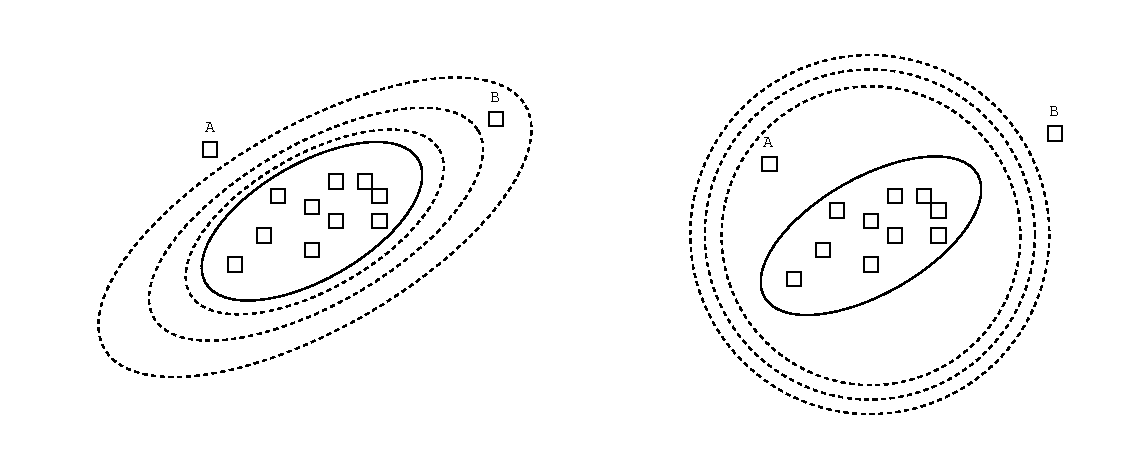
\includegraphics[width=0.8\textwidth]{img/maha.drawio.pdf}
    \caption{The comparison of the Mahalanobis (left) and Euclidean (right) distance in the context of elliptic clusters. The contour lines represent the space of the equal distance from the cluster centroid.}
    \label{fig:ellipses}
\end{figure}

Finally, Algorithm~\ref{alg01:maha} summarizes the Hierarchical Clustering (HC) with Mahalanobis linkage. Line~2 initiates $n-1$ iterations, each one starting with one less cluster to merge. Denoting $d$ as the dimension of the data, the time complexity of the Mahalanobis distance computation is $\mathcal{O}(d^2)$, according to the Equation~\ref{eq01:maha} and the fact, that the size of a covariance matrix is $d \times d$. The time complexity of the covariance matrix computation is $\mathcal{O}(d^2 \cdot c)$, where $c$ is the size of a cluster, and its inverse is computed in $\mathcal{O}(d^3)$. 

The standard HC, which utilizes a dissimilarity matrix, has a time complexity of $\mathcal{O}(n^3)$ and space complexity of $\mathcal{O}(n^2)$. There are other variants of HC, which influence the closest cluster pair retrieval and the amount of distances to recompute after each iteration. Other variants include HC with the nearest neighbor array, which trades the linear memory complexity for a worse time complexity on average, or the HC with priority queues, which reduces the time complexity to $\mathcal{O}(n^2 \log n)$ for the sake of bigger memory requirements~\cite{day1984efficient}. 

\begin{algorithm}[t]
    \caption{Mahalanobis Hierarchical Clustering Analysis}
    \label{alg01:maha}
    \begin{algorithmic}[1]
        \Procedure{MHCA}{Set of clusters $C = \{c_1, \dots, c_n\}$, dimension $d\in\N$}
        \While {$|C| > 1$}
            \For {all cluster pairs $(c_i, c_j)$}
                \State Compute $\delta_\text{Maha}(c_i,c_j)$ \Comment{Time: $\mathcal{O}(d^2)$}
            \EndFor
            \State Find the closest pair of clusters $(a, b)$
            \State Update $C$ by merging $a$ and $b$ into $c$
            \State Compute $\cov^{-1}(c)$ \Comment{Time: $\mathcal{O}(d^2 \cdot |c| + d^3)$}
        \EndWhile
        \EndProcedure
    \end{algorithmic}
\end{algorithm}

% We analyzed datasets with n = 10^4 events as the distance of data points requires O(n2) space in memory, and therefore, it becomes impractical (or even impossible) to analyze bigger datasets on current desktop computers.

% IN childhood acute lymphoblastic leukemia (ALL), response to therapy as measured by minimal residual disease (MRD) monitoring is an important biomarker for predicting relapse and stratifying treatment (1–5).

% , flow cytometry generates increasingly large and information-rich
% datasets, which provide new challenges for analysis. Modern multilaser flow cytometers are able to simultaneously measure up to 12 or more parameters and acquire
% such information from millions of single cells (8,9)

% Traditional gating of populations
% on two-parameter plots is tedious and does not reflect the multidimensionality of the data. Moreover, both the setting of the gates and interpretation of the results are observer-dependent and require intensive training and high levels of expertise. 

% Although hierarchical clustering methods
% can place each cell in its hierarchical context within the analyzed dataset, their downside is that they often fail to reflect
% the elliptical shapes of flow cytometric population

% However, the rapidly rising complexity of multiparameter
% flow cytometry datasets creates new challenges. Currently, the
% analytical standard in the field involves gating, in which one
% or more gates are defined in each histogram or dual parameter
% plot and a sequence or combination of gates defines the population of interest. This process is tedious or even unfeasible, already requires highly experienced cytometrists and is observer
% dependent. Most importantly, the sequential gating is limited
% in its ability to reflect the multidimensionality of the data. A
% solution to both the multidimensionality of flow data and the
% observer dependency lies in the usage of unsupervised learning
% methods.

% C version of the algorithm has been implemented within R package mhca and enhanced with the possibility of assuming
% apriori clusters for approximation, to reduce the unfavorable O(n3) time complexity for large datasets. That allowed the authors to process datasets of around
% 106 data points within an interactive environments



% problem - quadratic space complexity - even bigger problem with Mahalanobis distance and gpus 

\subsection{Implementation}



From the perspective of GPU programming, Mahalanobis HC is a challenging problem. Algorithms with a high memory requirements are generally unfavorable for GPUs due to their limited DRAM. There has been a lot of work on overcoming this limitation, both from NVIDIA and the scientific community~\cite{zheng2016towards,kim2020batch,landaverde2014investigation}. CUDA has introduced \emph{unified memory}~\cite{site:cuda}, which allowed GPUs to work on data that exceeds GPU memory capacity by seamlesly copying data from CPU to GPU on page fault. This optimization can help only to a certain extent, as it can only scale to the size of CPU RAM and the data are usually sent through high-latency small-throughput interconnect. Therefore, in our work we experimented with other well-known HC variants which trade higher time complexity for a linear memory complexity --- \emph{HC with the nearest neighbor array}~\cite{day1984efficient}. 
% Furthermore, the execution on the real-world flow cytometry data showed that the average cost of the nearest neighbor array update is much lower than the worst case.


The other obstacle of Mahalanobis HC is the greatly imbalanced workload. In the first iterations, the runtime is dominated by the complex Mahalanobis linkage computation over many pairs of $n$ clusters. But as the number of clusters decreases, the hot-spot becomes the computation of the covariance matrix of a merged cluster (Algorithm~\ref{alg01:esom}, Line~8). As a result, for the most time during the computation the GPU is not fully utilized either due to small amount of parallelism in covariance matrix computation or in the similarity computation. For that case, we designed a workload which uses CUDA \emph{streams}~\cite{site:cuda}, which are CUDA constructs that enable high-level GPU task parallelism, such as overlapping the execution of mutliple GPU kernels and memory transfers. Consequently, this allowed us to keep the utilization of more GPU cores during the whole runtime of the algorithm.

\subsection{Results}

As a result, the optimized Mahalanobis HC achieves a speedup of over $1400\times$ compared to the original serial CPU implementation. We benchmarked the application on the real-world single-cytometry datasets. The biggest dataset which we obtained, the Samusik-All~\cite{flowrepo} ($841$K $39$-dimensional points), was able to finish in the order of minutes compared to the order of days. Furthermore, the application has been distributed as a R package \texttt{gmhc} to fit workflows carrried out by a bioinformatics comunity. As of our knowledge, the package enabled the scientists to analyze big datasets as a whole, without the apriori clustering approximation, increasing the accuracy of the analysed data and decreasing the turnaround time of the analysis.  

% Hierarchical Clustering (HC) is a well-known problem, and there are many algorithms that effectively solve it. Roughly, they can be divided into categories according to the data structures they employ [TODO]:
% \begin{itemize}
%     \item HC with a dissimilarity matrix --- the most straightforward approach; the dissimilarity matrix stores the distances between all pairs of clusters. This approach has a cubic time complexity and quadratic memory complexity.
%     \item HC with a nearest neighbor array --- each cluster stores the index of its nearest neighbor. This approach trades a linear memory complexity for an asymptotic time complexity of $\mathcal{O}(d \cdot n^3)$.
%     \item HC with an array of priority queues --- a more sophisticated solution, which reduces the time complexity to $\mathcal{O}(n^2 \log n)$.
% \end{itemize}

% C application \texttt{mhclust}, the original implementation of the Mahalanobis HC, uses the dissimilarity matrix. This approach is simple and allows for a straightforward implementation. However, the empirical data reveal the most significant limiting factor in the quadratic memory complexity. The Mahalanobis distance adds a multiplicative factor in $\mathcal{O}(d^2)$ to the memory complexity, so usually, the machine runs out of memory before the execution time reaches unreasonable limits.

% As a solution to this limitation, we can assume \emph{in-place} variant of the HC with dissimilarity matrix, which discards the whole matrix and chooses the closest cluster pair by computing the distances ad-hoc. This increases the asymptotic time complexity to $\mathcal{O}(d \cdot n^3)$ assuming the Euclidean distance with centroid linkage.

% Our work used the nearest neighbor array approach to achieve fewer distance computations per iteration on average while keeping the memory complexity linear. Notably, the algorithm complexity per iteration is quadratic only in the worst case, when each cluster's neighbor needs to be reevaluated. This case would correspond to constantly merging such cluster pairs that all the other clusters are neighboring. In practice, this is an atypical case, and the empirical data show that the number of neighbors to reevaluate is generally in the range of 10 to 100 for tested datasets with at most 1M of points.

% Apart from the complex distance computation, the Mahalanobis HC suffers from the unbalanced nature of the algorithm. In the first iterations, the runtime is dominated by the distance computation in the data structure update. However, when the number of clusters decreases, the bottleneck becomes the covariance matrix computation of a merged cluster (with a time complexity of $\mathcal{O}(d^2 \cdot n)$). We used \emph{streams}, a CUDA abstraction for task parallelism on GPUs, to overlap the covariance matrix computation with the data structure update to keep GPU utilization high.

% \subsection{Future work}

% The Mahalanobis HC is a valuable method for analyzing cytometry data. However, since we published the optimized algorithm, there have been new additions to the GPU CUDA framework, which could be used to improve the performance of the algorithm further. Specifically, the whole Mahalanobis distance could be computed as a single \emph{Tensor} operation, drastically improving the application throughput. Another promising optimization would be to use \emph{CUDA Graph} to reduce the kernel launch overhead.


\section{Neighborhood-based dimensionality reduction}

% Another approach to the analysis of multidimensional point-like cloud datasets is to reduce the dimensionality of the data to a lower (human-readable) dimension while preserving the local structure of the data. This approach is used in many areas of life sciences, such as microscopy imaging, population biology, and others. The most popular methods for dimensionality reduction are t-SNE and UMAP. Both these methods are nonlinear neighborhood embeddings and use a stochastic approach to find the optimal mapping. However, their applicability reaches a limit when increasing the scale or requiring real-time processing.

% The EmbedSOM algorithm tries to tackle this limitation. It is based on self-organizing maps and uses a landmarks-based approach to reduce the computational complexity. Instead of computing all pairwise distances and stochastically optimizing the low-dimensional mapping, EmbedSOM uses a small set of landmarks to approximate the mapping. This allows for over a magnitude better performance while retaining the reasonable accuracy of the results. In our works, we followed up on the EmbedSOM algorithm and implemented it on GPUs to achieve real-time processing of large datasets, allowing for a semi-supervised dataset analysis.


Complementary to hierarchical clustering, a different approach to displaying cytometry datasets is \emph{dimensionality reduction} (also called \emph{embedding}), in which multi-dimensional cells are projected into a 2-dimensional plane, a picture, which shows cells arranged in groups with common properties. This methodology allows for a fast and reliable way to analyze cell populations, their relative size, and the presence of various features. The currently used dimensionality reduction tools are typically based on the principle of optimizing a low-dimensional embedding while preserving high-dimensional properties of interest. However, the most popular tools following this methodology, such as t-SNE~\cite{maaten2008visualizing}, UMAP~\cite{becht2019dimensionality} or TriMAP~\cite{amid2019trimap}, can suffer poor performance on large data due to the need to examine a nontrivial subset of $\binom{n}{2}$ relations (such as the pairwise distances) between $n$ data points~\cite{kratochvil2019generalized}.

A lot of effort has been dedicated to optimizing the performance of these algorithms. Solely for t-SNE, we can find multiple works related to this topic~\cite{pezzotti2016hierarchical,pezzotti2016approximated,linderman2017efficient,belkina2018automated}. Regardless of these developments, the processing time of these algorithms scales super-linearly with the number of data points, which inevitably leads to the need of data downsampling. \emph{EmbedSOM} algorithm, introduced by Kratochvíl et al.~\cite{kratochvil2019generalized}, is designed to overcome this limitation. The costly parts of the previous methods can be omitted by creating a smaller model of the data obtained (not exclusively) by \emph{self-organizing maps}. EmbedSOM uses the information of such an approximated manifold to compute the final embedding, retaining a competitive quality of the visualization. 

Algorithm~\ref{alg01:esom} shows the overview of EmbedSOM. It assumes a set of $n$ high-dimensional points $X \in \R^{n \times d}$ and the smaller data model: a set of $g << n$ high-dimensional landmarks $L \in \R^{g \times d}$, and a set of $g$ low-dimensional landmarks $l \in \R^{g \times 2}$. For each input point, $k < g$ nearest landmarks from $L$ are found and assigned scores according to their distance. Finally, we compute the embedding such that the difference between distances from $l$ landmarks and the embedded point and $L$ landmarks and the original point is minimized. The minimization problem is reducible to a linear system of equations with two variables.

\begin{algorithm}[t]
    \caption{EmbedSOM}
    \label{alg01:esom}
    \begin{algorithmic}[1]
        \Procedure{EmbedSOM}{$X\in\R^{n\times d}$, $L\in\R^{g\times d}$, $l\in\R^{g\times 2}$, $k\in\N$}
        \For {$i \in \{1\dots n\}$} \Comment{For each high-dimensional point}
            \State Find $k$ nearest landmarks from $L$
            \State Score the $k$ nearest landmarks according to the distance to $X_i$ with $s_1, \dots, s_k$
            \For {$(u,v) \in \{1,\dots,k\}^2$ } \Comment{For each pair of nearest landmarks}
                \State Compute $D_{uv}(X_i)$ by projecting $X_i$ orthogonally onto a line between $L_u$ and $L_v$; We define $d_{uv}(x)$ similarly for $l_u$ and $l_v$
            \EndFor
            \State Find $x_i$, such that $\sum_{u, v} s_u \cdot s_v \cdot (D_{uv}(X_i) - d_{uv}(x_i))$ is minimized
        \EndFor
        \EndProcedure
    \end{algorithmic}
\end{algorithm}

With such a description of the algorithm, we can deduce the time complexity for a single data point processing: The first line of the for loop is the well-known $k$-NN problem, with the optimal time complexity of $\mathcal{O}(d \cdot g \cdot \log k)$. The remainder, which we may call the embedding step, has a time complexity of $\mathcal{O}(d \cdot k^2)$. Since it holds that $k < g << n$, EmbedSOM achieves sufficient scaling; the embedding of $24$ million cells with $36$ markers can finish under an hour on common hardware, compared to around $2$ days using UMAP~\cite{kratochvil2019som}. Figure~\ref{fig:embedsom} visualizes the EmbedSOM process.

\begin{figure}[h]
    \centering
    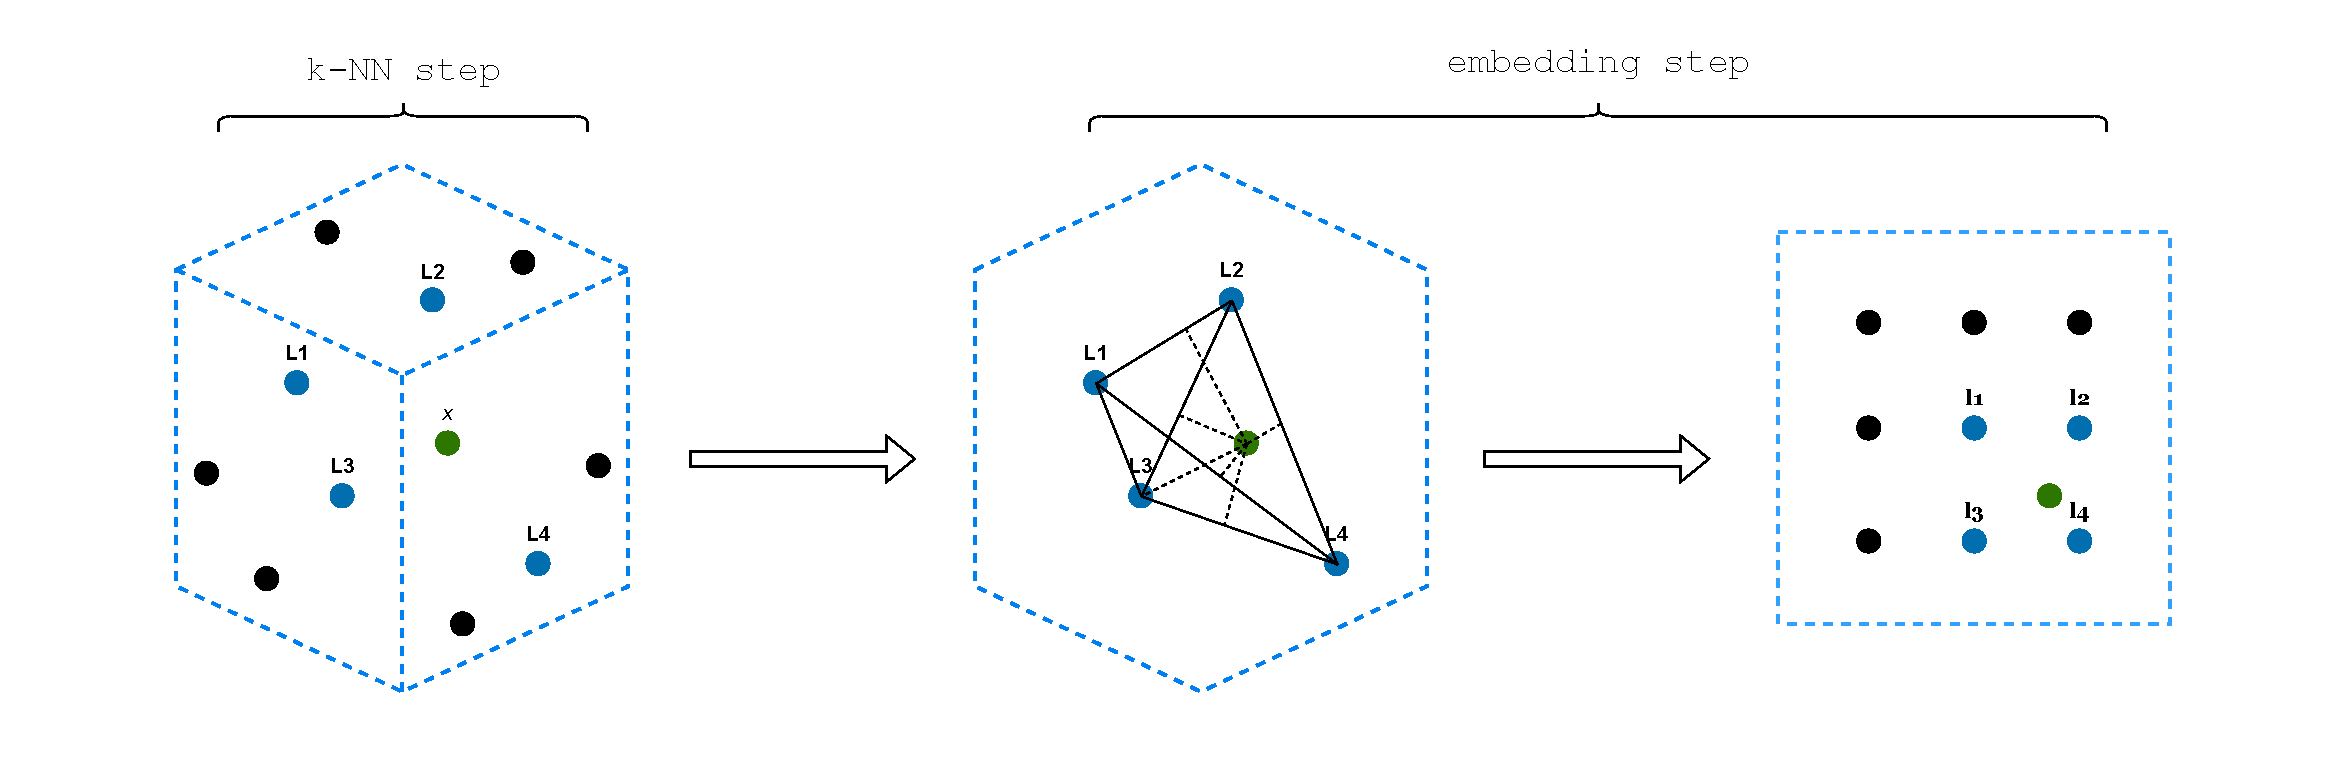
\includegraphics[width=\textwidth]{img/embedsom.drawio.pdf}
    \caption{The visualization of the EmbedSOM algorithm, with $k$-NN and embedding steps highlighted.}
    \label{fig:embedsom}
\end{figure}

\subsection{Interactive opportunities of GPU implementation}

Although the EmbedSOM CPU implementation already provided good performance, it still had an untapped parallelization potential and a potential for enablement as an interactive method in cytometry data analysis. Therefore, we followed up on it in our work. 

The main challenge of EmbedSOM is low \emph{arithmetic intensity} --- the number of math operations per transferred byte. A huge math bandwidth of a GPU can only be achieved if the device can keep up transferring data from memory to the cores. Low arithmetic intensity indicates that data transfers will not keep up with the math bandwidth.

Note that although the arithmetic intensity is primarily determined by the algorithm, it can be influenced by its implementation in a major way. For GPUs, there are many ways to fight the arithmetic intensity of an algorithm, such as kernel fusion~\cite{wahib2014scalable}, leveraging the memory hierarchy~\cite{lee2012cuda} or by reordering data accesses~\cite{ghysels2012improving} and optimizing data transactions~\cite{lu2020optimizing}. Generally, these approaches can be distilled into two groups:
\begin{itemize}
    \item \emph{Data reuse} --- A single datum is reused for as many operations as possible. This is especially useful for algorithms that load the same data multiple times for different computations. 
    \item \emph{Latency hiding} --- Instead of waiting for data to arrive, a GPU context-switches to different threads to perform other operations. GPUs are designed to schedule many more threads than the number of cores with very little overhead. With enough work overlapping, the high memory latencies can be completely hidden.
\end{itemize}

We experimented with both approaches in our EmbedSOM implementation. Although caches can partially handle data reuse, GPUs typically hardly benefit from them due to their low cache-to-core ratio~\cite{site:cuda}. Therefore, as one variant of $k$-NN part, we used \emph{shared memory}, a programmable cache, to store the data and landmarks. These were then used to compute all the possible pairwise distances before loading the next batch to maximize the arithmetic intensity. The second variant of the $k$-NN part used a highly parallel \emph{bitonic sort} to find the top-$k$ landmarks. This approach has the hidden benefit of low per-thread resource requirements, resulting in higher maximum GPU occupancy and, consequently, better latency hiding.

The embedding part of EmbedSOM does not offer such a data reuse opportunity, as each point has a different set of nearest landmarks. The only reuse can happen on the landmarks themselves. And since their count can be limited in some parameter configurations, we experimented with techniques that increase the memory bandwidth, such as \emph{vector load instructions}. 

\subsection{Results}

After the thorough benchmarking process, we selected the most performing variants of both steps and combined them into a complete implementation of the EmbedSOM algorithm. We increased the performance by $200-1000\times$ over the serial CPU version and $3-10\times$ over a naive GPU implementation. Furthermore, the achieved speedup enabled the interactive data visualization and was integrated into the graphical application \emph{BlosSOM}~\cite{molnarova2023throughput} (see Figure~\ref{fig:blossom}). Thanks to the added performance, the application can project datasets of up to a million points with a maintained frame rate above $30$ frames per second on consumer hardware. This contribution pushes the boundary of EmbedSOM into a semi-supervised dimensionality reduction domain, allowing users to effectively and intuitively visualize data with real-time feedback.

\begin{figure}   
    \centering
    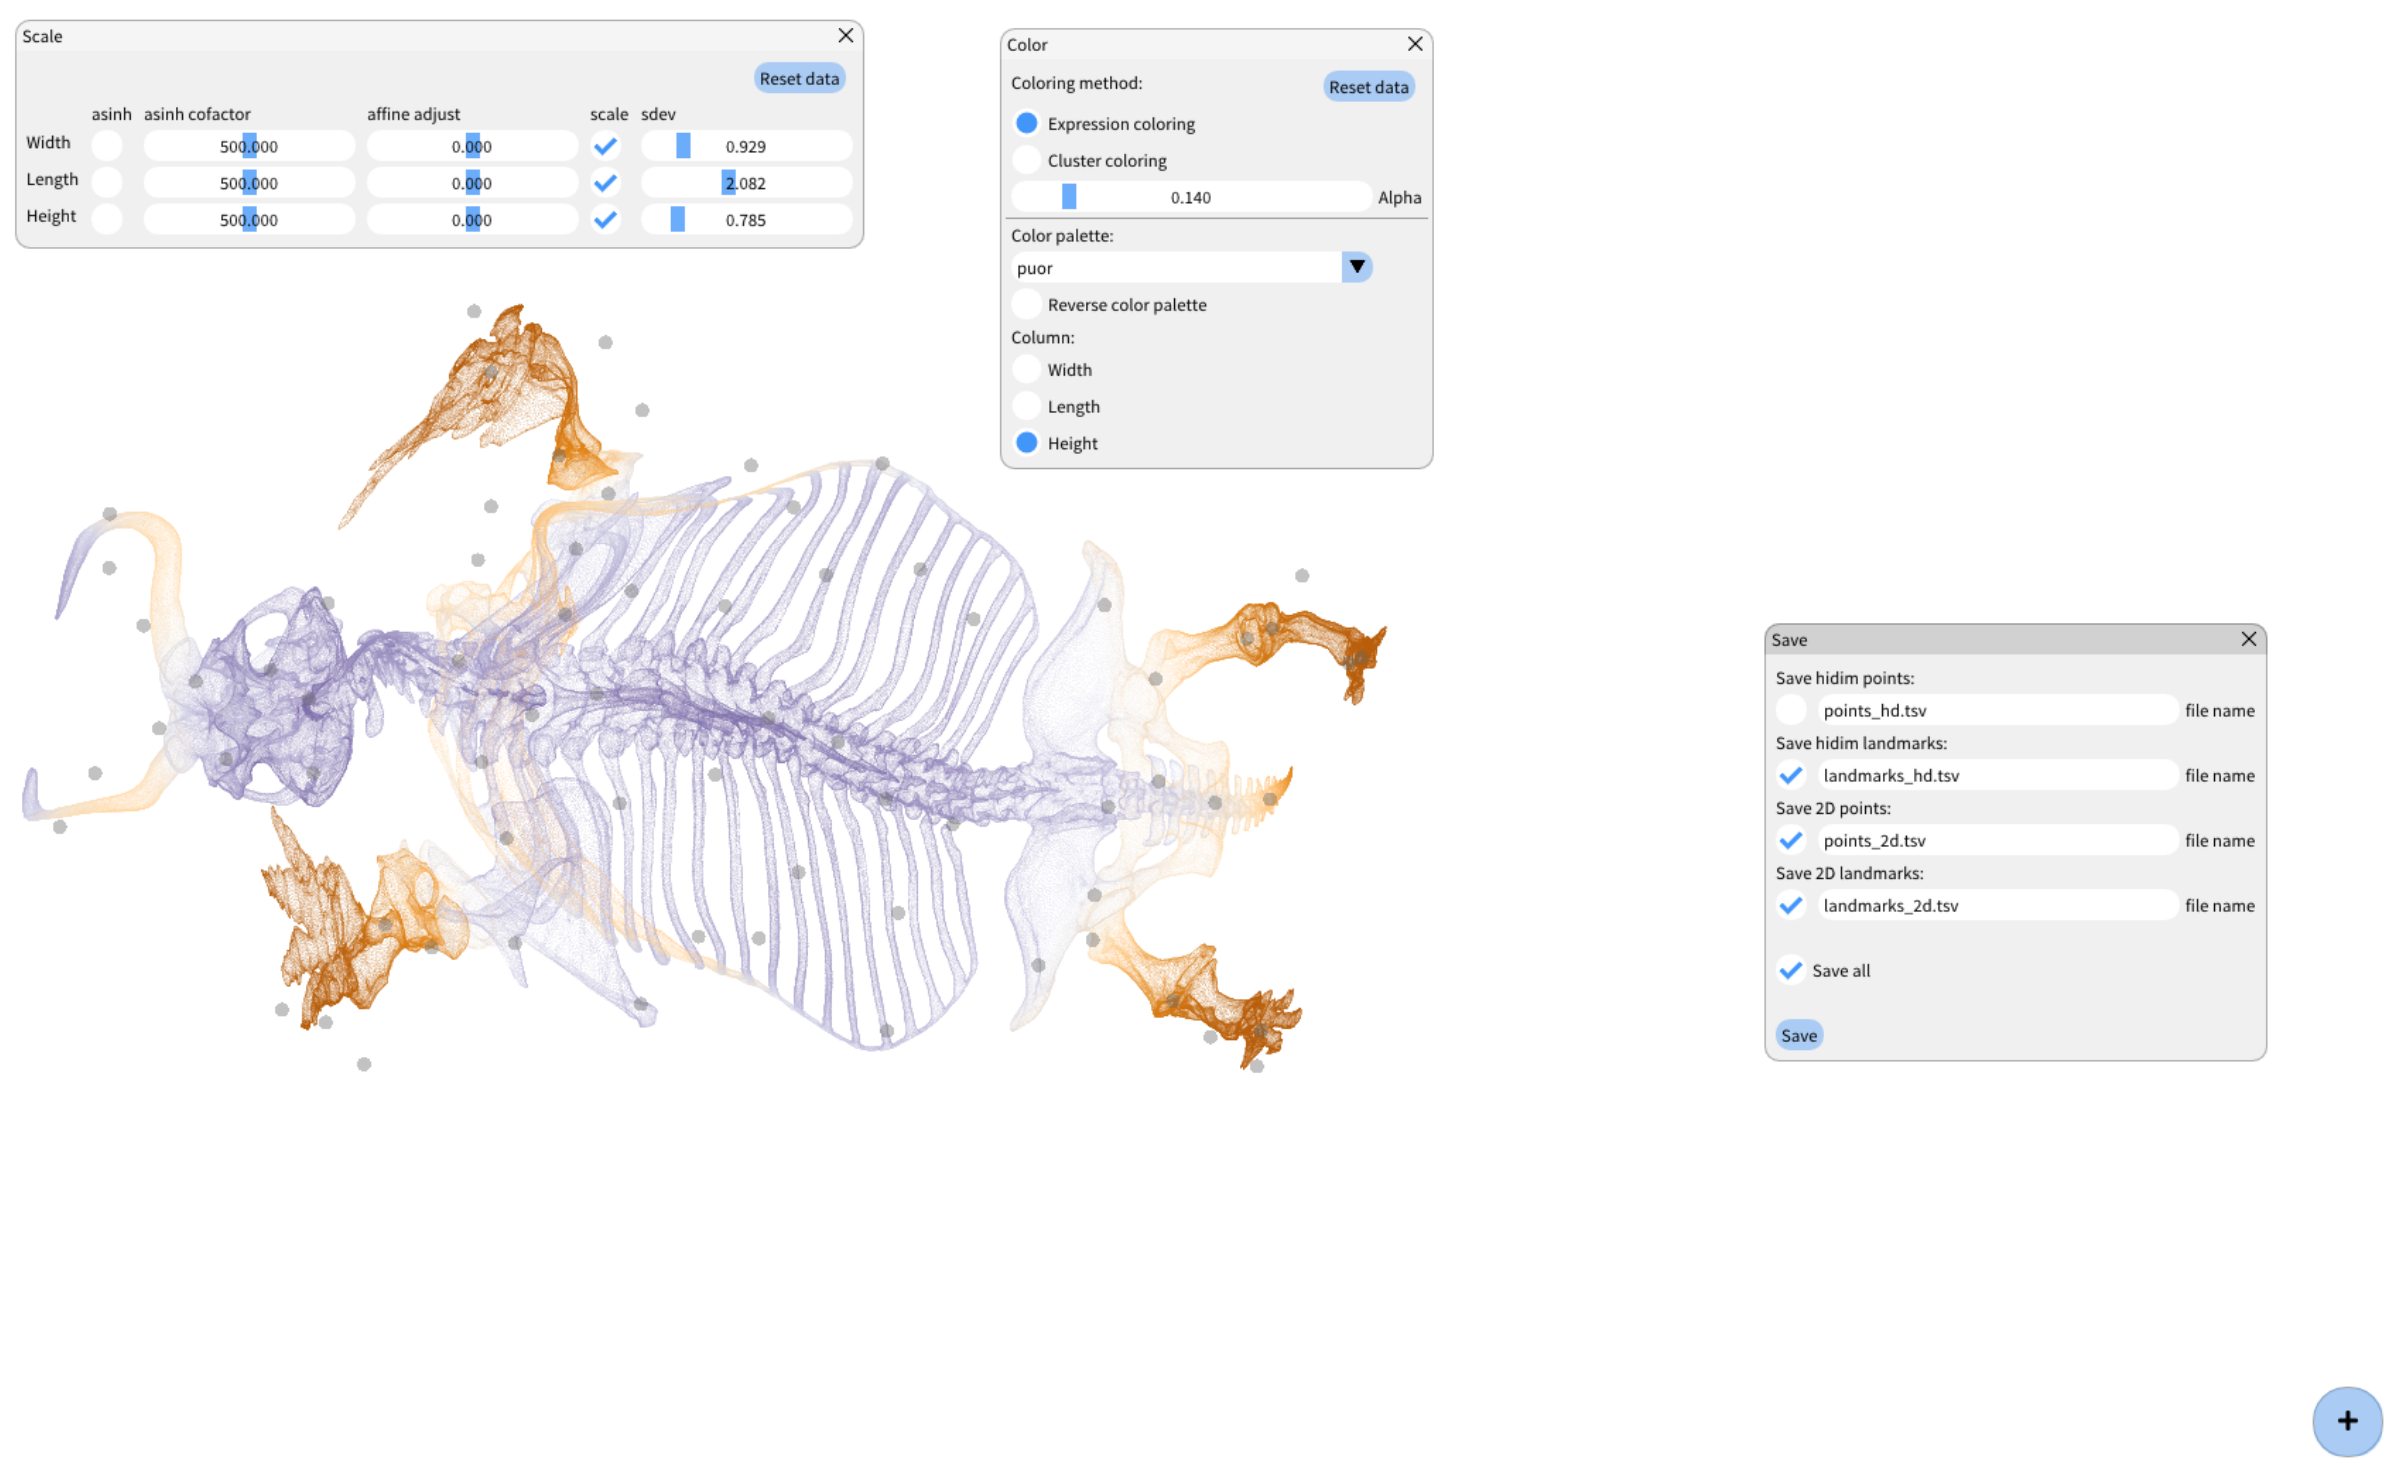
\includegraphics[width=0.7\textwidth]{img/blossom.png}
    \caption{Mammoth skeleton dataset visualized in BlosSOM.}
    \label{fig:blossom}
\end{figure}

% EmbedSOM projection can be viewed as an embedding enrichment method: From a set of landmarks in the 
% high-dimensional space and a set of corresponding landmarks in the low-dimensional space, it produces a smooth 
% function that maps all points from the higher-dimensional space to the low-dimensional space and preserves 
% the relative neighborhoods of the landmarks. EmbedSOM was originally designed to work with simple SOMoriginating landmarks, as shown in Figure 1.

% Ecient unbiased data analysis is a major challenge for laboratories handling
% large ƒow and mass cytometry datasets. We present EmbedSOM, a non-linear
% embedding algorithm based on FlowSOM that improves the analysis by providing high-performance embedding method for the cytometry data. ‘e algorithm
% is designed for linear scaling with number of data points, and speed suitable for
% interactive analysis of millions of cells without downsampling. At the same time,
% the visualization quality of single cell distribution within cellular populations and
% their transition states is competitive with the current state-of-the-art algorithms.
% We demonstrate EmbedSOM properties on two use-cases, showing bene€ts of using the interactive algorithm speed in supervised hierarchical dissection of cell
% populations, and the scalability improvement by eciently processing very large
% datasets.

% ‘e ever-increasing size and dimensionality of data generated by ƒow and
% mass cytometry experiments drive interest in simplifying data analysis. Employing the usual repetitive manual gating, exploration and back-gating techniques is tedious if the sample count is high, and becomes imprecise on complex
% 20 data. During the past decade, a multitude of automated analysis methods have
% been introduced, including various unsupervised clustering and phenotyping algorithms, and embedding methods. Comprehensive reviews of the algorithms
% are available [19, 27, 10, 11]

% The preferred method to display cytometry datasets is embedding, in which
% 25 cells are arranged into a 2-dimensional picture showing populations of agglomerated cells with similar properties. ‘is provides a straightforward way to inspect
% the relative population sizes, their contents, and the presence of various features
% including major subpopulations, intermediate cell states and trajectories of their
% development. ‘e performance of available embedding algorithms is constantly
% 30 being improved. For example, the widely used tSNE [24] has formed the basis
% for faster ASNE [17] and HSNE [16], and was further improved in OptSNE and
% FItSNE [3, 14] and accelerated using GPU by Chan et al. [5]. Other methods include SWNE, scvis, largevis [29, 6, 8], and the relatively new UMAP [15] that
% speci€cally aims to provide be‹er, faster embedding than tSNE. Despite these
% 35 developments, two key objectives have not been met:
% • ‘e embedding algorithm should be able to process the data of volumes
% common in cytometry quickly, ideally within seconds, to allow interactive
% data inspection;
% • algorithm processing time should scale linearly with the number of cells,
% 40 to be able to keep up with the increasing sizes of datasets without downsampling.
% We introduce EmbedSOM, a new embedding algorithm that is designed to
% satisfy these two requirements. ‘e algorithm uses a self-organizing map (SOM)
% that describes the multidimensional cell space. SOMs have been successfully
% 45 used for classifying this space into clusters — for example, FlowSOM [25] uses
% SOM vertices as cluster centers to classify the cells into clusters that form a basis
% for further analysis. ‘e SOM additionally approximates a section of a smooth
% 2-manifold embedded in the multidimensional space in a manner such that the
% cells are uniformly distributed in its neighborhood. EmbedSOM uses this addi50 tional information to compute the embedding by €‹ing a projection of each cell
% 2
% onto this manifold, and transforming the projection coordinates to 2-dimensional
% SOM-relative coordinates.
% ‘e performance-oriented design of EmbedSOM di‚ers substantially from
% other commonly used embedding methods. Most importantly, the usual time55 consuming iterative optimization of single cell positions in the embedding is replaced by relatively fast manifold approximation by SOM training. Additionally,
% the separation of the SOM-training from other stages of the algorithm introduces ƒexibility that allows precise manipulation of separate embedding properties, such as reliable alignment of cell populations in the embedding even with
% 60 substantially di‚erent samples, and easy optimization of the embedding layout

% 2.1. EmbedSOM provides superior embedding speed
% ‘e main distinctive feature of EmbedSOM is its computational eciency. A
% dataset of common size (approximately 300k cells and 20 markers) can be mapped
% by the SOM and embedded in less than a minute; the GPU-accelerated versions of
% the algorithms deliver the same result in seconds. Generally, embedding datasets
% 80 with millions of cells and several dozen markers is possible in minutes using
% common oce hardware. Moreover, since the major SOM-training part of the
% required computation is shared with FlowSOM, EmbedSOM visualization adds
% only minor computational complexity to workƒows that already use FlowSOM.
% antitative measurements of the speed advantage on the benchmark com85 putations are displayed in Figure 1a. ‘e results con€rm the expected performance scaling gap between UMAP and EmbedSOM, caused by di‚erent algo3
% rithm design. Generally, UMAP and tSNE are very ecient for high-dimensional
% data with a low data point count, because they remove the dimensionality overhead early in the process but require more than linear amount of computation
% 90 to optimize the €nal data point positions. ‘e performance of both EmbedSOM
% stages is linear in the number of data points, but the dimensionality overhead is
% present throughout almost the entire computation as another linear factor.
% EmbedSOM bene€ts from this trade-o‚ when applied to high-volume ƒow
% and mass cytometry data that are physically limited to dozens of dimensions.
% 95 Conversely, UMAP remains faster on low-volume datasets with more than hundreds of dimensions. For example, the raw single-cell RNA sequencing data must
% be pre-processed (e.g. reduced to principal components) in order to deliver comparable results with SOM-based algorithms [7].
% Overall, the performance scaling di‚erence is best illustrated by the compu100 tation time required for running workƒows used later in the article: Embeddingassisted dissection of 1 million cells (Section 2.3) takes less than 5 minutes of
% computation with EmbedSOM; but more than 1 hour with UMAP. Embedding of
% the 24 million cells from Pregnancy dataset (Section 2.4) can be €nished faster
% than in 1 hour with EmbedSOM, but requires around 2 days with UMAP.

% The SOM is used for multiple purposes: an embedded single-cell
% view of the samples is computed from the SOM using the fast
% EmbedSOM algorithm (Kratochvı´l et al., 2019). Clustering of the
% cells is conducted in an interactive dendrogram (Sieger et al.,
% 2017) built from hierarchical metaclustering of the SOM content.
% Notably, ShinySOM supports the agglomerative clustering with
% Mahalanobis-average linkage (Fiser et al., 2012) that has been
% shown to be capable of defining cell populations with the same accuracy as expert cytometrists in a real life setting. After selecting the
% cell populations, the user may display and analyze the differences
% between samples and sample groups, and visualize the results of
% statistical testing of the differences in cell abundance. Finally, the
% annotated populations may be partitioned into smaller datasets, in
% order to be explored in more detail.


\section{Cross-correlation optimized for small inputs}

Leaving the realm of cytometry data analysis, we will focus on a highly data-bound problem: cross-correlation. This algorithm is a cornerstone of many scientific fields, such as image processing, seismology, material physics, and, with the advent of convolutional neural networks, machine learning. As one interpretation, it computes a similarity of two data series obtained by sliding one over the other and computing the dot product of the overlapping parts. The output is typically post-processed to get richer information, such as Earth's underground structure~\cite{zhou2021high} in seismology, road lane detection~\cite{fan2018real} in computer vision, or acoustic location~\cite{belloch2015performance} in signal processing.

The problem of cross-correlation performance was initially introduced to us by the physicists from the Department of Physics of Material at Charles University in Prague. They used the algorithm to analyze the diffraction pattern of metallic alloys from electron backscatter diffraction (EBSD) cameras to obtain the material \emph{deformation}. That can be used to study the material characteristics, such as elastic strain or lattice rotation.

A typical input consists of a \emph{reference} 2D grayscale image of the analyzed material and multiple images of the \emph{deformed} material (as depicted in Figure~\ref{roi-shifts}). In the $1:N$ relation, the reference image is cross-correlated with each deformed image to find the most similar shift, which suggests the direction of deformation. However, different parts of the image may be deformed differently. Therefore, images are typically divided into smaller parts, and the cross-correlation is computed for each part separately, requiring multiple $1:N$ cross-correlations. Considering such input configuration, the computation can quickly get expensive, and the analysis becomes performance-constrained.

The reference Python script provides the physicists with the computational throughput of tens of patterns per second. However, modern EBSD cameras produce data at a magnitude higher rate~\cite{bali2021zpracovani}. Nevertheless, thanks to the parallel nature of the problem, this is a perfect candidate for GPU acceleration. 

\begin{figure}[h]
	\centering
	\begin{subfigure}{.33\textwidth}
		\centering
		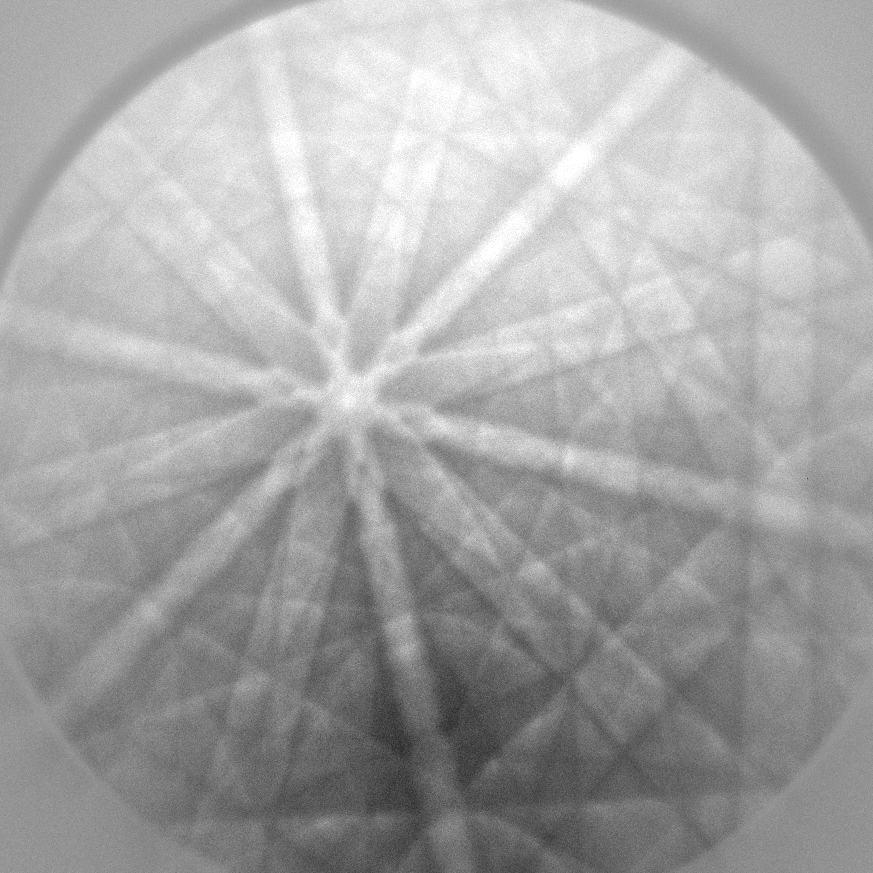
\includegraphics[width=.6\linewidth]{img/roi_shifts_initial}
		\caption{Reference pattern}
		\label{roi-shifts:initial}
	\end{subfigure}%
	\begin{subfigure}{.33\textwidth}
		\centering
		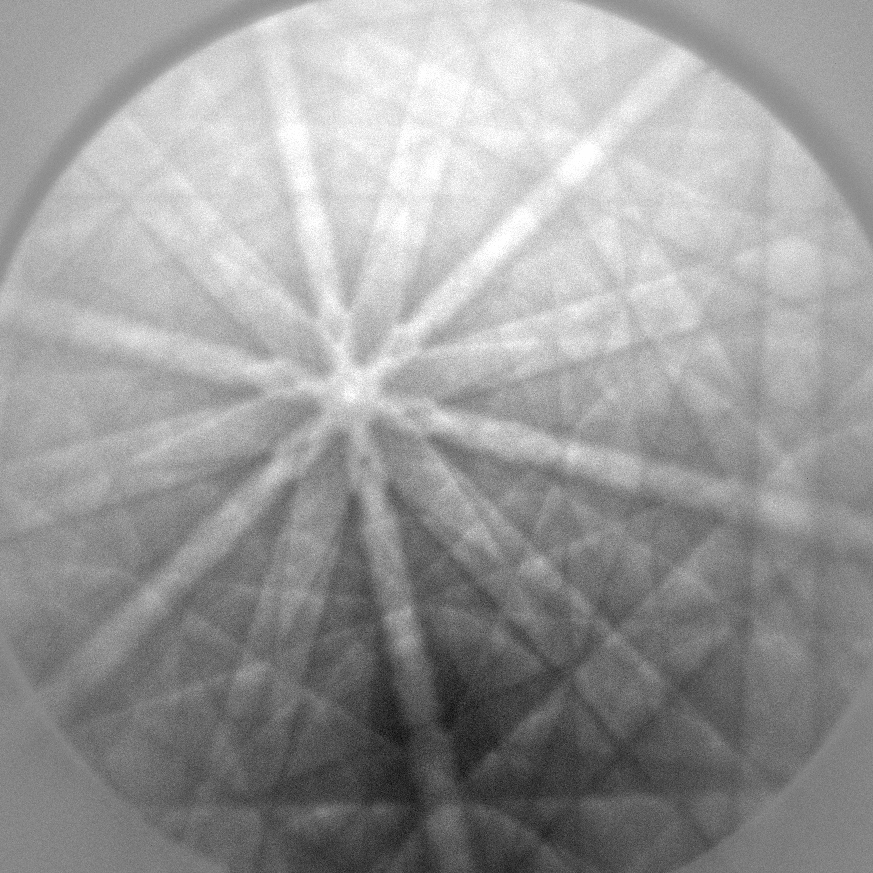
\includegraphics[width=.6\linewidth]{img/DEFORMED_x3600y6235}
		\caption{Deformed pattern}
		\label{roi-shifts:deformed}
	\end{subfigure}
	\begin{subfigure}{.33\textwidth}
		\centering
		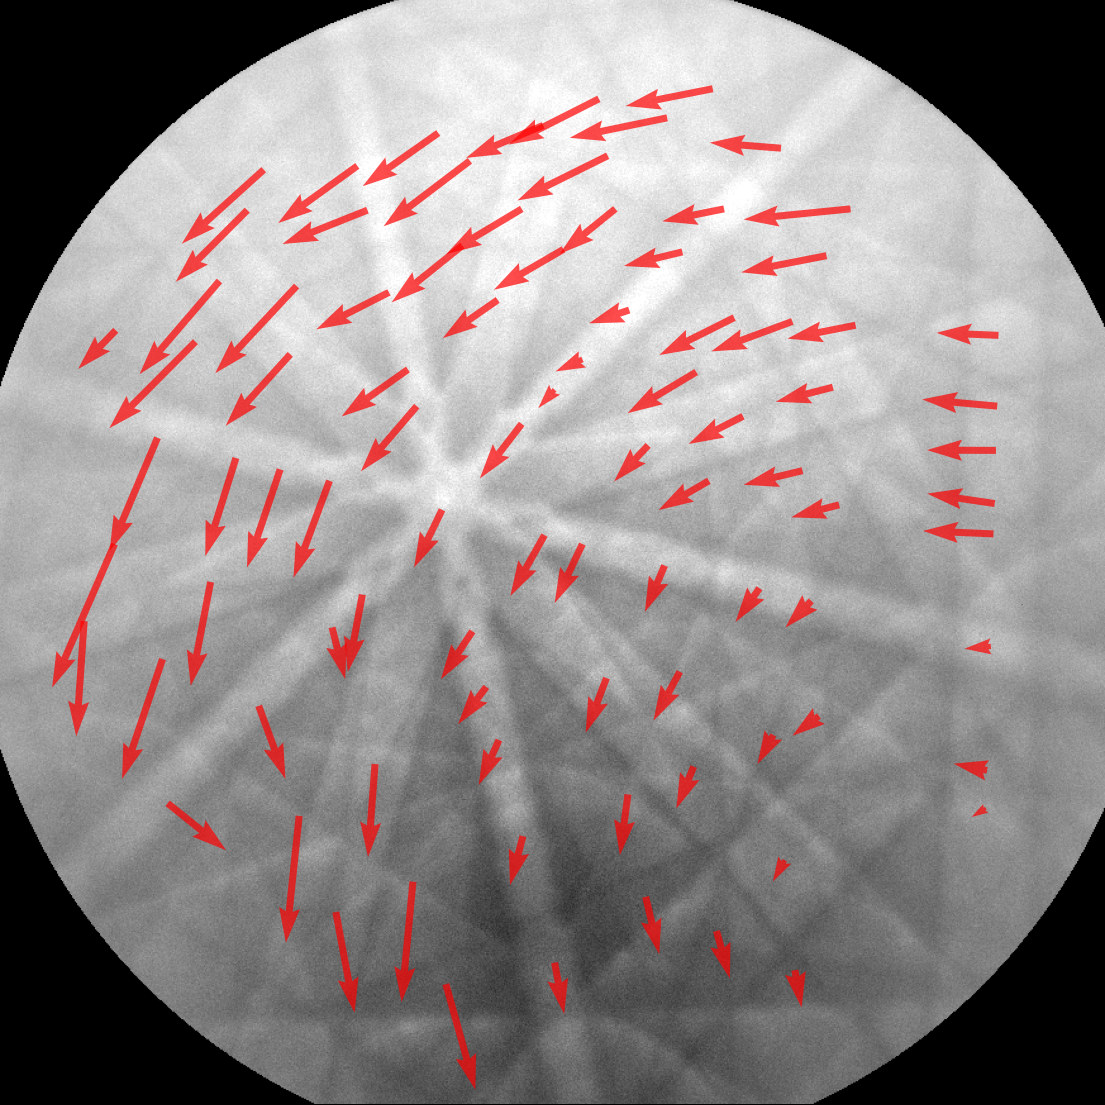
\includegraphics[width=.6\linewidth]{img/roi_shifts}
		\caption{Deformation visualization}
		\label{roi-shifts:result}
	\end{subfigure}
	
	\caption{A visualization of FeAl alloy deformation computed using cross-correlation}
	\label{roi-shifts}
\end{figure}

\subsection{Implementation challenges}

The cross-correlation of functions $f, g: \mathbb{C}\rightarrow \R$ is defined as
\begin{equation}
    (f \star g)(\tau) = \sum_{i=-\infty}^{\infty} f(i) g(i+\tau).
\end{equation}
Figure~\ref{fig:cross-correlation} depicts the visual representation of the equation applied on a discrete case of two $2\times 2$ matrices. The matrices are shifted to produce all the possible overlaps (Figure~\ref{fig:cross-correlation}, right). For a single shift, only overlapping elements contribute to the computation: overlapped pairs are multiplied and summed together into a single output matrix element (Figure~\ref{fig:cross-correlation}, left). From the perspective of the implementation, a trivial solution is achieved rather quickly by defining four nested loops, two for the shift and two for the overlap computation as shown in Listing~\ref{lst:cross}.

\begin{figure}
    \centering
    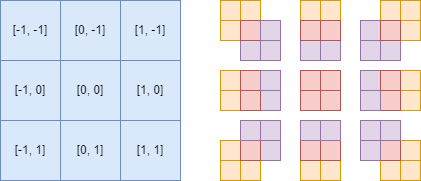
\includegraphics[width=0.6\textwidth]{img/cc.png}
    \caption{Visual representation of the cross-correlation. Yellow and purple matrices correspond to the input matrices, and the blue matrix depicts the cross-correlation output. The coordinates on the blue matrix correspond to the shift of the yellow matrix, which is depicted on the right. Only the overlapping parts (in pink) contribute to the computation for each output matrix element.}
    \label{fig:cross-correlation}
\end{figure}

For general $w \times h$ matrices, the cross-correlation has a time complexity of $\mathcal{O}(w^2 \cdot h^2)$. Alternatively, the input can be modified and passed to the Fast Fourier Transform (FFT) with a more pleasing time complexity of $\mathcal{O}(w\cdot h \cdot \log(w\cdot h))$. However, the hidden multiplicative factor, which materializes as an overhead in the implementations of FFT, favors the original, definition-based approach for small problem sizes.

\begin{listing}
\begin{minted}[fontsize=\footnotesize,breaklines]{c++}
for (int i = -(n - 1); i <= n - 1; i++)
    for (int j = -(n - 1); j <= n - 1; j++)
        for (int y = 0; y < n - abs(i); y++)
            for (int x = 0; x < n - abs(j); x++)
                result[j][i] += a[max(0, -i) + y][max(0, -j) + x] * 
                                b[max(0,  i) + y][max(0,  j) + x];
\end{minted}
\caption{A trivial implementation of cross-correlation.}
\label{lst:cross}
\end{listing}

To assess the optimality of the trivial implementation, let us compute the arithmetic intensity of a single overlap computation. For $n$ overlapped element pairs, we need to perform $n$ fused multiply-add operations. Considering the elements are represented as $4$B single-precision floating points, the arithmetic intensity equals to $\frac{n}{2n * 4} = \frac{1}{8}$. To get a notion of the ideal value for the best hardware utilization, modern profilers include the \emph{roofline model}~\cite{williams2009roofline}. It is a graphical representation of a hardware attainable performance, given the algorithm arithmetic intensity.

Another helpful metric, especially for GPUs, is to obtain the \emph{ops per byte} ratio~\cite{site:cudaopb}. It is computed as the ratio of math and memory bandwidth, and when compared with an arithmetic intensity, it indicates whether the bottleneck lies in the arithmetic or memory pipeline. To put it into perspective, the ops per byte ratio of a modern NVIDIA V100 GPU is around $17$ for single-precision floats (and if we consider the \emph{tensor-cores}, optimized for matrix multiplication, ops per byte ratio is up to $67$). Since $\frac{1}{8} < 17$, the implementation of such an algorithm will be highly memory-bound.

\subsection{Optimization techniques}

With this in mind, we experimented with extreme data-sharing techniques. There are many opportunities where the same data is read multiple times:
\begin{itemize}
    \item When computing neighboring overlaps, most data from left and right matrices are read multiple times.
    \item In the $1:N$ scenario, when cross-correlating one left matrix with many right matrices, the data from the left matrix is read multiple times when computing the same overlap between multiple right matrices.
    \item In the $N:M$ scenario, multiple left and right matrices can be read once to compute overlaps between all of them.
\end{itemize}

With such techniques, the arithmetic intensity is theoretically unbounded, provided an infinitely big input. However, the physical resources limit the practical values of the reuse factor. The most important resource is the register file. In order to reuse data, threads need to have them stored in the registers. The number of registers is limited, and the compiler can spill the data into slower memory if the limit is reached. Also, if the amount of resources per thread is high, the occupancy of the GPU can drop, and the achievable performance can decrease. 

The other big issue is the parallelism. Naturally, if one worker performs multiple operations for the sake of sharing, the parallelism decreases. Therefore, the most effective implementation maintains the optimal balance between data sharing and parallelism.

Lastly, the memory hierarchy can aid a low arithmetic intensity: the memory bandwidth is inversely proportional to the ops per byte ratio. If most of the working data resides in the faster memory, the ops per byte ratio is lower, and less computing is required to saturate the memory bandwidth. For the L2 cache of NVIDIA V100, the ops per byte ratio is around $3.5\times$ less than for the off-chip memory. As a result, if the caches are utilized correctly, less data sharing is required to utilize the hardware capabilities fully.

In our implementation, we took GPU-specific advantage of even faster memory than L2, the register file itself, to cache the data. The GPU register file is rather big, having $64$KB of capacity. However, the caching possibilities on thread registers are very limited. They are only allowed on a group of $32$ consecutive threads called a warp and allow only a specific access pattern. Still, they provide a higher throughput than the closest cache, the shared memory.

\subsection{Results}

The final implementation of the cross-correlation algorithm achieved a speedup of $5-10\times$ over a naive GPU code. The benchmark also uncovered the boundaries, above which a more expensive time complexity of the definition-based algorithm overcomes the overhead of the FFT approach. In summary, achieved speedup can enable physicists to analyze the data at a similar rate as EBSD cameras produce.


\section{Stochastic simulation of Boolean networks}

% Large and complex biological systems. 
% Represented as boolean networks. Vertices represent states and edges transition between states. 
% Transitions from a state are described by boolean formulas on the states.

% Analythical methods are limited to small models. (power of two)
% Simulated as Monte Carlo simulations.

% Bigger models require a lot of simulations. Sizek takes a non trivial amount of time. There are bigger models. Mutant analysis is even more expensive. Restricted to single mutants 

% A tough problem for GPU - iterating binary tree brings a lot of branching, a lot of memory accesses, a lot of data to transfer.
% branch divergence, memory access patterns are of concern
% could be solved by different methods - no collaboration of boolean formuals - reduce divergence
% - reduce memory access - store the data in a different way

% Or we can use cuda nvrtc to compile the boolean formulas on the fly. This would allow us to remove the memory access. Added compilation step amortized in the bigger and longer simulations.

% We enabled solbing big models in matters of milliseconds. now, consumer laptop can simulate models that were previously restricted to high-end computers. we can think about not jsut single Mutant analysis (also double tripple), python wrapper is being developed.

In Systems biology, the analysis of large and complex biological systems is a challenging task. \emph{Boolean models}~\cite{wang2012boolean} have gained popularity due to their simplicity, scalability, and ability to describe complex signaling networks. A Boolean model consists of $n$ nodes with binary values --- active or inactive. A node represents an event in the system, such as a gene being expressed or a protein being activated. The complete state of the system is, therefore, defined by a boolean word composed of $n$ bits. The states can transition within each other based on $n$ Boolean formulae, one for each node. Given an initial state, the task of the model is to predict the probability distribution of system outcomes after a specified amount of time.

Numerical methods, such as ExaStoLog~\cite{koltai2020exact}, have been developed and used to solve Boolean models; however, they are limited to relatively small models (tens of nodes) due to the exponential memory requirements. For larger models, it has proved to be much more efficient to approximate the results by simulation. A C++ software, MaBoSS~\cite{stoll2017maboss}, simulates these systems by applying the kinetic Monte-Carlo algorithm~\cite{stoll2012continuous} on the Boolean network. In summary, the MaBoSS tool simulates millions of random walks (also called the \emph{trajectories}) on the state space of the Boolean network (a directed weighted graph). Algorithm~\ref{alg:iter} shows in a higher-level how a trajectory is sampled. The trajectories are then aggregated in a histogram-like fashion to compute various statistics, such as the probability distribution of the states over time, as is shown on Figure~\ref{fig:maboss}.

\begin{algorithm}
    \caption{A single iteration of the MaBoSS simulation of a trajectory, given the trajectory state $S$ at time $t$.}
    \label{alg:iter}
    \begin{algorithmic}[1]
    \Procedure{TrajectorySimulationStep}{S, t}
    \State Compute transition probabilities $p_1, \dots, p_n$ by evaluating the Boolean formulae $\mathcal{B}_1, \dots, \mathcal{B}_n$ on $S$
    \State Sample the next state $S'$ and transition time $\Delta t$ according to the probabilities $p_1, \dots, p_n$
    \State \Return $S'$, $t + \Delta t$ 
    \EndProcedure
    \end{algorithmic}
\end{algorithm}

Due to the stochastic nature, this approach can overcome the limitations of numerical methods and has enabled the analysis of bigger models, running instances with a few hundred nodes in a reasonable amount of time. On the other hand, allowing even bigger inputs would require billions of simulated trajectories in order to obtain a reliable result, which puts significant pressure on the tool and its ability to scale well. A parallel CPU MaBoSS simulation of a relatively small Sizek model~\cite{sizek2019boolean} ($n=93$) with $10^6$ trajectories takes the order of minutes on a high-end computer. Simulating models with thousands of nodes and billions of trajectories would require an order of days in runtime, hindering further analysis of the models.

\begin{figure}
    \centering
    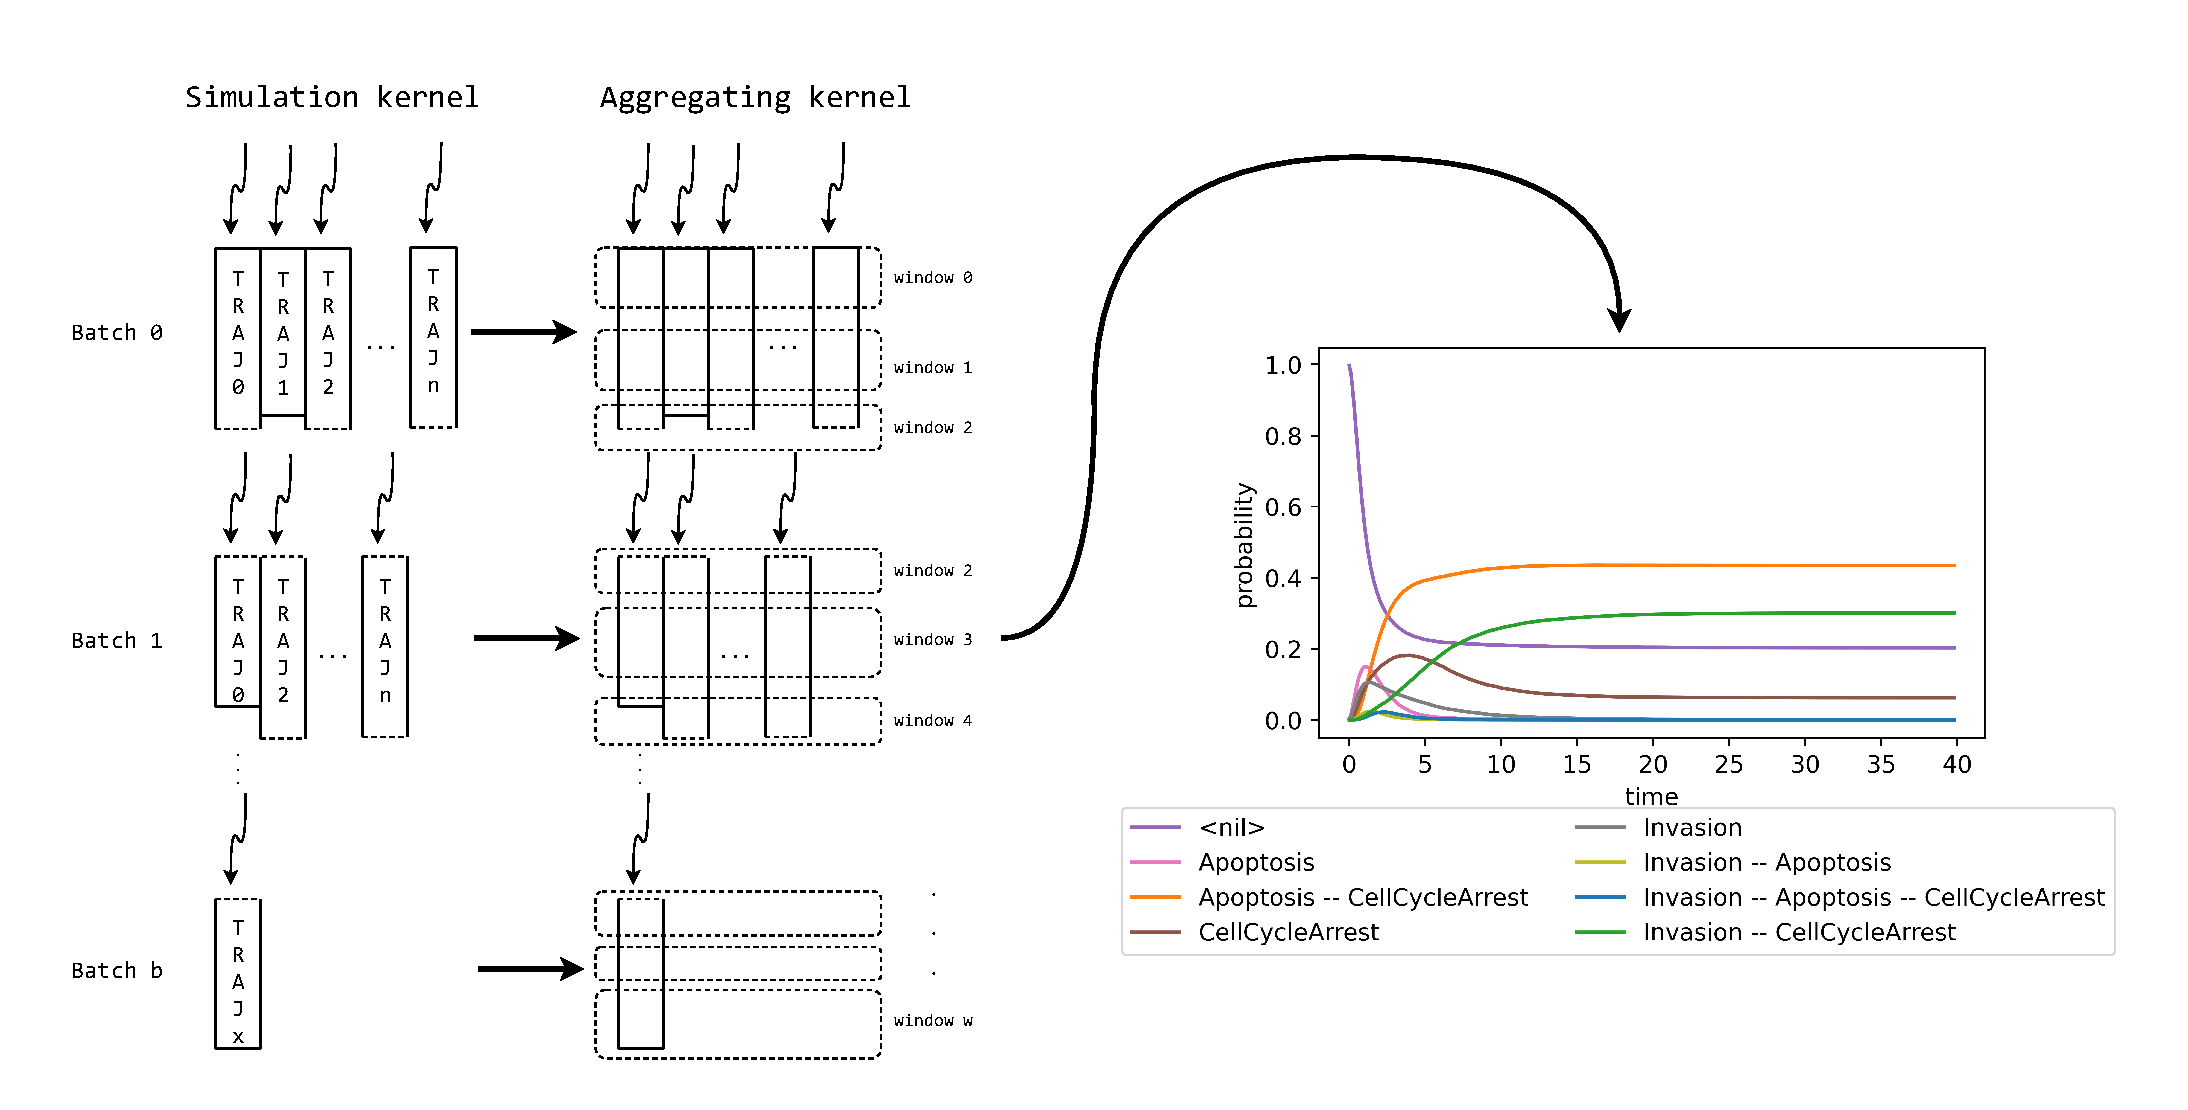
\includegraphics[width=\textwidth]{img/mabossg-kernels.drawio.pdf}
    \caption{The MaBoSS projection of simulated trajectories averaged over a specific time window.}
    \label{fig:maboss}
\end{figure}

Another performance challenge is the so-called \emph{mutant analysis}. In an existing model, a node is \emph{mutated} to a static value, losing the ability to change its state. This technique is used to predict the effect of a gene knockout or overexpression. During the analysis, the same model is run $2n$ times to gain the predictions of each single mutation (both suppressed and expressed). Naturally, this sort of analysis is even more expensive. As a result, the analysis of double or triple mutants (where multiple nodes are mutated at once) has been subjected to a supercomputer-level task.


\subsection{GPU acceleration challenges}

Although the parallelization of MaBoSS may seem straightforward, it includes challenges that can significantly affect the overall performance. The main issue is the traversal of the binary expression tree to evaluate the Boolean formulae. Generally, traversing irregular data structures causes conditional branching and creates an irregular data access pattern. The latter ineffectively utilizes memory transactions, reducing the memory bandwidth, which is a crucial factor for GPU performance, as stated in the previous sections. Moreover, executing divergent branches on GPUs can be punished by serial execution of the threads if the branch divergence happens on the warp level. A combination of these issues may leave GPU heavily underutilized, gaining very little to no performance improvement over a well-parallelized CPU code.

Branch divergence can be mitigated by cleverly distributing formulae evaluations among the threads. The most straightforward approach is to assign all $n$ formulae computations to a single thread such that the threads execute the same formula in each step. The divergence within the evaluation of the same formula can be solved by turning off short-circuiting optimization and enforcing the threads always to evaluate the whole expression. 
The other possible approach would be to assign one formula to a thread. Naturally, this enables more parallelism but requires a more complex data structure to prevent thread divergence. The formulae need to be represented in the code so that each of their execution is issued as the same sequence of instructions. A way to achieve this is to convert formulas to CNF or DNF form and store them in the memory as a vector of bitmasks with a unified length.

In our work, we partly followed the first approach. But instead of designing an ideal memory layout for the formulae, we used the \emph{CUDA NVRTC}~\cite{nvrtc-online} runtime compilation library to compile the formulas on the fly. It has the benefit of encoding the formulas into a native binary code, removing the necessity to fetch the data from the memory each time the formula is evaluated. Apart from that, the compiler can run a set of optimizations on the code, further improving the performance. Consequently, the runtime compilation comes at the cost of an additional runtime. Thankfully, our benchmarking showed that the compilation time amortizes well for simulations with reasonably big inputs.

\subsection{Results}

The final implementation of the MaBoSS simulation achieved a speedup of $100-300\times$ on real-world datasets over the parallel CPU version. Moreover, we created a synthetic test suite to stress the scalability of the implementation, which showed that the GPU implementation can simulate models with thousands of nodes and billions of trajectories in minutes. These results suggest that the consumer laptop equipped with a GPU can simulate models that were previously restricted to high-end computers. Furthermore, the double and triple mutant analysis no longer belongs just to the domain of supercomputers but could become feasible on data center-grade GPUs. Overall, we believe that the GPU acceleration of the MaBoSS simulation can significantly improve the analysis of Boolean networks and enable researchers to explore complex models while conveniently using their personal computers.



% thesis is organized as follows

% tam pridat paragraf ku kazdemu clanku

% a az na koniec 1

% viac zrovnanie

% preco su tieto alg tazke

% pitfally co sa stanu ked implementujes na gpu

% v inter tiez dokladne povedat preco to mame rozdelene na scientific aglos + noarr



% gPu science
% - ukazat preco je to zaujimave
% - ze to je potrebne pre biologov
% - ze to zlepsuje situaciu pre vyskum
% - ze je to zaujimavy problem - takze asi spomenut ake boli doterajsie limitacie
% - ukazat ze to je fakt tazky - popisat, co si to vyzadovalo, ake to malo problemy, ma to vela moznosti kde to paralelizovat, vsetky popisat 
% - ale na vysokej urovni - zhrnut a vysvetlit ze to je tazke
% - na zaver poplacat na zadech - zrychlili sme to 1000x

% - future work skor nie 
% - 

% ku intur hodit referencie idealne surveye


% vypychnut trochu viac algoritmy - odstavec o algoritme
% zahodit preface
% namiesto part 2 apendix
% do GPU intro pridat tie najvacie problemy skrz gpu optims a v sekciach sa na ne odkazovat
% to otvori dvere aj conclusion - urcim tie najvacsie problemy, poviem ako pomalsia je pamat wrt compute
% bibliography za part 1 a nie az za clanky
% obrazok ku kazdemu clanku (mozno graf do results, mozno pre lepsiu vizualizaciu problemu)
% viac citacii - najma v intre